\documentclass[12pt]{article}

\usepackage{sbc-template}

\usepackage{graphicx,url}
\usepackage{float}

%\usepackage[brazil]{babel}   
\usepackage[utf8]{inputenc}  

     
\sloppy

\title{Unikernel}

\author{Eduardo Henrique Mendel\inst{1}, Gabriel Porto dos Santos\inst{1}, Guilherme Gonçalves\inst{1}}


\address{
  Escola Politécnina- Universidade do Vale do Rio dos Sinos\\
  93022-750 -- São Leopoldo -- RS -- Brazil
  \email{\{gaporto\}@edu.unisinos.br}
} % Colocar ", [usuário]" entre os "{}"

\begin{document} 

\maketitle

% \begin{abstract}

% \end{abstract}
     
% \begin{resumo} 

% \end{resumo}


\section{Introdução}

Em relação aos Sistemas Operacionais modernos, a virtualização, contemporaneamente, mostra-se como um tópico imprescindível para o desenvolvimento de aplicações dada a ênfase na conteinerização e modularização de aspectos de infraestrutura em realidades como a \textit{IoT}, por exemplo. Devido a tópicos como este, há a utilização de funcionalidades destes por meio de \textit{Cloud} ou módulos embarcados a fim de aumentar suas possibilidades de um dado sistema. Todavia, esta abordagem possui um problema intrínseco: a complexidade do Kernel do sistema que a mantém. No caso do Linux, seu Kernel é relativamente flexível, mas em determinados contextos onde é empregado pode vir a se tornar um problema quanto a performance e portabilidade.

A fim de sobrepor situações não benéficas relacionados a este problema estrutural, emprega-se o \textit{Unikernel}. Este é definido por ser uma abordagem por intermédio de bibliotecas específicas de componentes do sistema operacional que provém as mesmas a aplicação requerente da funcionalidade \cite{raza:196}, tornando-se ordens de grandeza mais eficiente quando comparado a uma virtualização completa e literal do sistema operacional utilizado.

O conceito fundamenta-se, basicamente, da utilização do sistema operacional semelhante ao uso de uma biblioteca - como por exemplo o \textit{mirageOS}. Vários módulos são carregados por intermédio de determinadas camadas de abstração que, dependendo de seu objetivo, são carregadas de forma mais eficiente no ambiente que a requer. Deste modo, esta "granulação" da arquitetura de um sistema operacional impede que o mesmo trate processos de modo a utilizar ferramentas para o tratamento multitarefa dos mesmos. O que ocorre é a compilação do mesmo a fim de proporcionar sua execução como processo único, tendo seu funcionamento e organização em geral semelhante a de um microsserviço \cite{fraga:120}.

\section{Arquitetura}

Em seu cerne, Unikernels são estruturados para funcionarem baseados na necessidade do sistema, isto é, o mesmo carateriza-se por ser orientado a serviço (\textit{service-based}). Desta forma, sua organização e arquitetura fundamentam-se em melhor atender a estas necessidades baseadas no módulos requeridos, utilizando uma abordagem cirúrgica em comparação ao modelo de virtualização de um sistema operacional ou outras abordagens, como visto na figura ~\ref{fig:fig1}.

\begin{figure}[H]
\centering
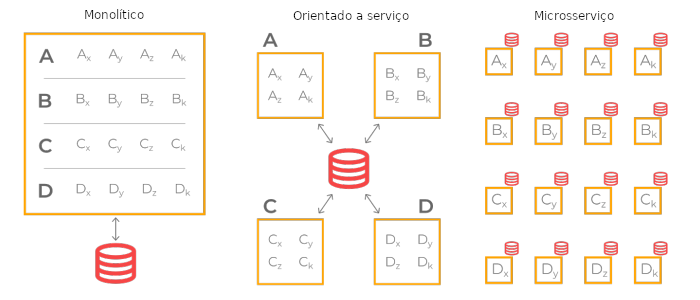
\includegraphics[width=.8\textwidth]{fig1.png}
\caption{Comparação das abordagens \cite{fraga:120}}
\label{fig:fig1}
\end{figure}

 Na mesma figura, utilizando como comparação a utilização de um banco de dados, exemplifica-se que a "granulação", diferente de uma alternativa mais monolítica de um sistema operacional ou orientada a serviço,módulos de Unikernel são um "universo próprio". 
 
 Isto é, não há dependências e por consequência \textit{overheads} geradas pela utilização de certos recursos


\bibliographystyle{sbc}
\bibliography{sbc-template}

\end{document}
